\documentclass{article}
    \author{杨铭\\5130379022}
    \title{Homework - Canny Edge Detector}
\usepackage{ctex}
\usepackage{graphicx}
\begin{document}
    \maketitle
    \section{简述}
        \paragraph{}主要代码在canny.py中,使用python编写,调用了python的copy库来做输出数组的深度复制,以及opencv的python
    接口实现对各种格式图像的读取和写入
    \section{输入格式}
        \paragraph{}使用opencv的cv2.imread函数读取图片,支持.bmp,.jpg.png等格式
    \section{实现方式}
        \paragraph{完成了canny边缘检测算法的一下四个步骤}
            \begin{itemize}
              \item Gaussian Blur
              \item Compute magnitude of gradient
              \item Non-maxima suppression
              \item Hysteresis thresholding
            \end{itemize}
        \paragraph{Gaussian Blur}高斯模糊,调用opencv库函数,使用的是3X3的结构体进行模糊\\
        \paragraph{Compute magnitude of gradient}用差分算子遍历图中每个像素,算出它们的横向梯度、纵向梯度和总梯度,并保存在三个数组中\\
        \paragraph{Non-maxima suppression}非极大值抑制

            \subparagraph{算法}
                根据上一步算出的梯度值,算出梯度方向,然后在梯度方向上查找该点是否为局部最大值。如果是,则保留,否则删掉。这一步可以删除大多数非边缘点
        \paragraph{Hysteresis thresholding}
            双阈值二值化
            \subparagraph{算法}用Otsu算法并取其返回值的1/3为低阈值,2/3为高阈值
        \section{结果}
            \paragraph{}
                \begin{figure}[htbp]
                    \begin{minipage}[t]{0.5\linewidth}\centering
                    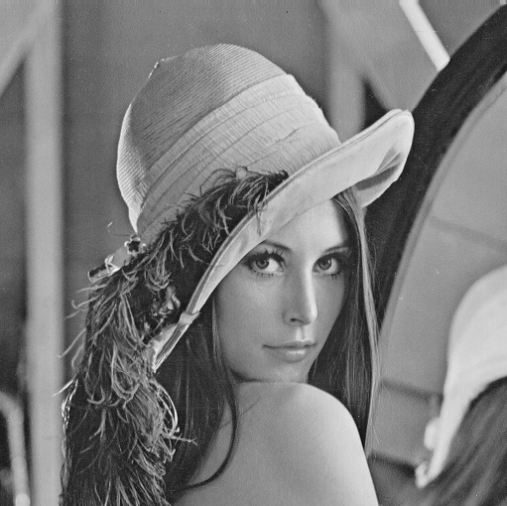
\includegraphics[width=6cm]{test.png}
                    \caption{原图}\label{1-a}
                    \end{minipage}
                    \begin{minipage}[t]{0.5\linewidth}\centering
                    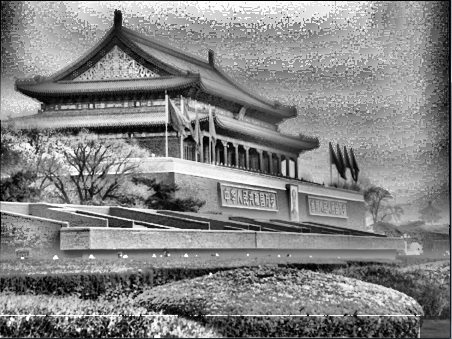
\includegraphics[width=6cm]{result.png}
                    \caption{边缘}\label{1-b}
                    \end{minipage}
                \end{figure}
            \paragraph{分析}
                算梯度值时使用的差分算子太过简单,导致不同点的梯度相差不够大,在双阈值处理时,我的取阈值方法并不标准,导致一些细节被忽略,而且边缘略显粗糙。不过总体效果比较满意。
\end{document}
